% Source for landing/public/thumbs/thumb-spde.png (card: Split SPDE-GMRF inference for lane perception).
% Build: landing/diagrams/build.sh thumb-spde
\documentclass[border=14pt]{standalone}
\usepackage{amsmath,amssymb}
\usepackage{tikz}
\usetikzlibrary{arrows.meta,positioning,fit,backgrounds,calc}
\definecolor{grp}{HTML}{B5B5B0}
\definecolor{exp}{HTML}{2E8B57}
\begin{document}
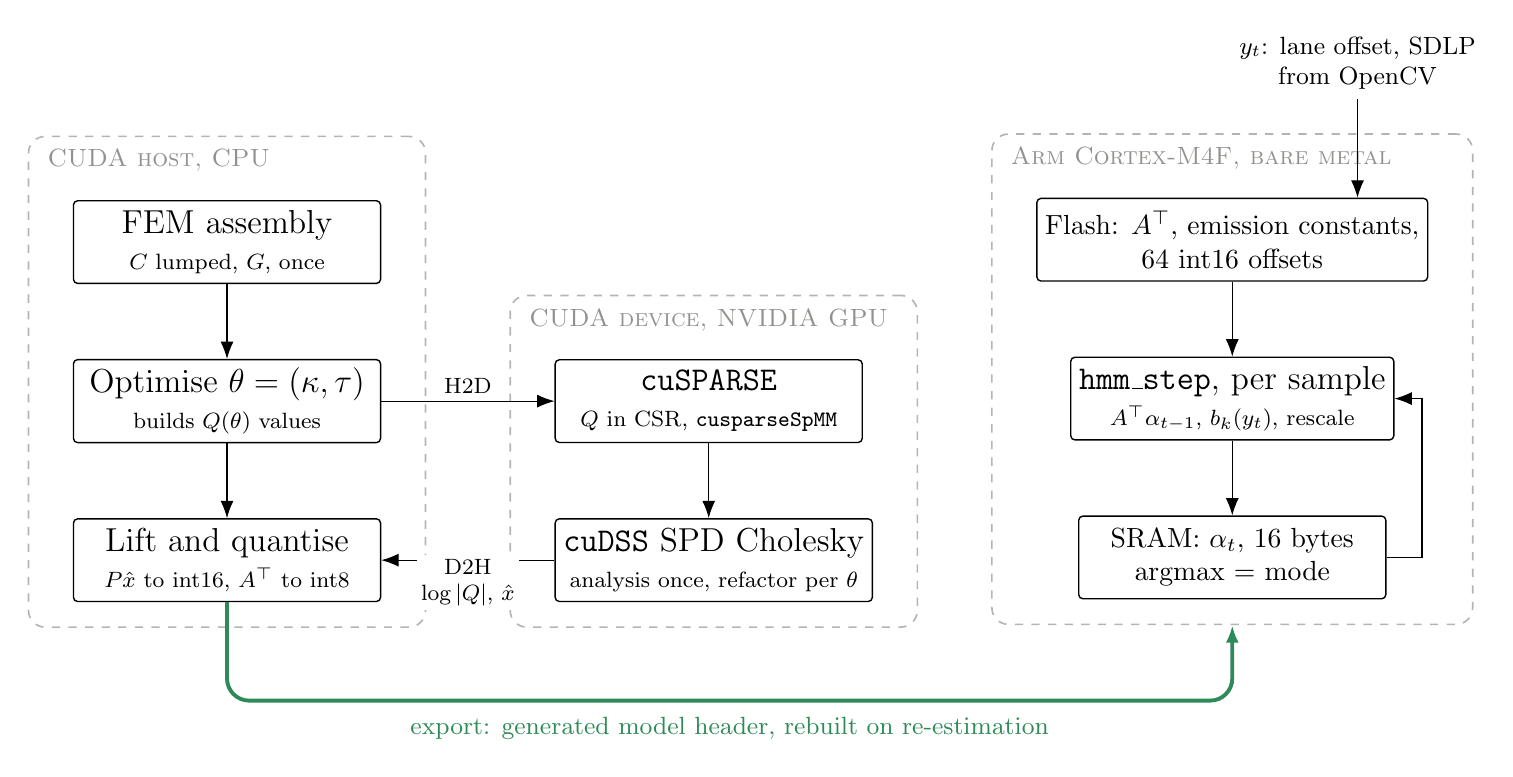
\begin{tikzpicture}[
  >={Latex[length=2.2mm]},
  box/.style={draw=black, fill=white, rounded corners=1.5pt, line width=0.5pt,
              minimum width=3.9cm, minimum height=1.05cm, align=center, inner sep=3pt},
  grp/.style={draw=grp, dashed, rounded corners=6pt, line width=0.6pt, inner sep=9pt, inner xsep=16pt},
  gl/.style={text=grp!80!black, font=\scshape\small, anchor=north west, inner sep=2pt, xshift=5pt, yshift=-3pt},
  sub/.style={font=\footnotesize},
  lbl/.style={font=\footnotesize, fill=white, inner sep=1.5pt},
]
% CUDA host
\node[box] (fem) at (0,0) {\large FEM assembly\\[1pt]{\footnotesize $C$ lumped, $G$, once}};
\node[box, below=0.95cm of fem] (opt) {\large Optimise $\theta=(\kappa,\tau)$\\[1pt]{\footnotesize builds $Q(\theta)$ values}};
\node[box, below=0.95cm of opt] (lift) {\large Lift and quantise\\[1pt]{\footnotesize $P\hat{x}$ to int16, $A^{\top}$ to int8}};
% GPU
\node[box, right=2.2cm of opt] (sp) {\large\texttt{cuSPARSE}\\[1pt]{\footnotesize $Q$ in CSR, \texttt{cusparseSpMM}}};
\node[box, right=2.2cm of lift] (chol) {\large\texttt{cuDSS} SPD Cholesky\\[1pt]{\footnotesize analysis once, refactor per $\theta$}};
% Cortex-M4F
\node[box, right=2.2cm of sp, yshift=2.05cm] (flash) {Flash: $A^{\top}$, emission constants,\\64 int16 offsets};
\node[box, below=0.95cm of flash] (hmm) {\large\texttt{hmm\_step}, per sample\\[1pt]{\footnotesize $A^{\top}\alpha_{t-1}$, $b_k(y_t)$, rescale}};
\node[box, below=0.95cm of hmm] (sram) {SRAM: $\alpha_t$, 16 bytes\\argmax $=$ mode};
\coordinate (yin) at ($(flash.north east)+(-0.9,0)$);
\node[above=1.25cm of yin, align=center, font=\small] (yt) {$y_t$: lane offset, SDLP\\from OpenCV};

\begin{scope}[on background layer]
  \node[grp, fit=(fem)(lift), yshift=7pt, inner ysep=16pt] (g1) {};
  \node[grp, fit=(sp)(chol), yshift=7pt, inner ysep=16pt] (g2) {};
  \node[grp, fit=(flash)(sram), yshift=7pt, inner ysep=16pt] (g3) {};
\end{scope}
\node[gl] at (g1.north west) {CUDA host, CPU};
\node[gl] at (g2.north west) {CUDA device, NVIDIA GPU};
\node[gl] at (g3.north west) {Arm Cortex-M4F, bare metal};

\draw[->] (fem) -- (opt);
\draw[->] (opt) -- (lift);
\draw[->] (opt) -- node[lbl, above=1pt] {H2D} (sp);
\draw[->] (sp.south) -- (sp.south |- chol.north);
\draw[->] (chol) -- node[lbl, align=center, below=-2pt] {D2H\\$\log|Q|$, $\hat{x}$} (lift);
\draw[->] (yt.south) -- (yin);
\draw[->] (flash) -- (hmm);
\draw[->] (hmm) -- (sram);
\draw[->] (sram.east) -- ++(0.45,0) |- (hmm.east);
\draw[->, exp, line width=1.4pt, rounded corners=8pt]
  (lift.south) -- ($(lift.south)+(0,-1.25)$) -| node[pos=0.25, below=2pt, font=\small, text=exp] {export: generated model header, rebuilt on re-estimation} (g3.south);
\end{tikzpicture}
\end{document}
